%
% Thesis template conforming to Williams College rules.
% Thanks to Ben Wood '08 and other contributors.
%
\documentclass[twoside]{report}
\usepackage[top=1.0in, bottom=1in, left=1.5in, right=1in, includehead]{geometry}
\pagestyle{headings}
\usepackage{setspace}
%% Special math fonts and symbols
\usepackage{amssymb}
\usepackage{amsfonts}
\usepackage{amsmath}
\usepackage{amsthm}
%% Rotate tables and figures
\usepackage{rotating}
%% Used for TODO items
\usepackage{xcolor}
%% used for code listings.
\usepackage{float} 
%% Used to replace LaTeX's ugly emptyset with diameter, which looks nicer.
\usepackage{wasysym}
%% Nicely formatted algorithms.
\usepackage{algorithmicx}
\usepackage[chapter]{algorithm}
\usepackage{algpseudocode}
%% Nicely formatted listings.
\usepackage{listings}
%% More kinds of arrow with stuff

\usepackage{empheq}
\usepackage{multicol}
\usepackage{subfigure}
\usepackage{indentfirst}
%% 
%% Hughes additions
%%
%% set table width
\usepackage{array}
%% graphics path
\graphicspath{{./figs/}}
%% hyperlinks
\definecolor{color1}{RGB}{0,0,90} % Color of the article title and sections
\definecolor{color2}{RGB}{0,20,20} % Color of the boxes behind the abstract and headings
\usepackage{hyperref} % Required for hyperlinks
\hypersetup{hidelinks,colorlinks,breaklinks=true,urlcolor=color2,citecolor=color1,linkcolor=color1,bookmarksopen=false,pdftitle={Title},pdfauthor={Author}}
%% Used to set up better TODO items
% \usepackage[paperwidth=210mm,
%             paperheight=297mm,
%             left=50pt,
%             top=50pt,
%             textwidth=345pt,
%             marginparsep=25pt,
%             marginparwidth=124pt,
%             textheight=692pt,
%             footskip=50pt]
%            {geometry}
\usepackage{xargs}

\newcommand{\halpha}{H$\alpha$}
\newcommand{\todo}[1]{{\color{red}{\textbf{#1}}}}

%\usepackage[colorinlistoftodos,prependcaption,textsize=tiny]{todonotes}
%\newcommandx{\unsure}[2][1=]{\todo[linecolor=red,backgroundcolor=red!25,bordercolor=red,#1]{#2}}
%\newcommandx{\change}[2][1=]{\todo[linecolor=blue,backgroundcolor=blue!25,bordercolor=blue,#1]{#2}}
%\newcommandx{\info}[2][1=]{\todo[linecolor=OliveGreen,backgroundcolor=OliveGreen!25,bordercolor=OliveGreen,#1]{#2}}
%\newcommandx{\improvement}[2][1=]{\todo[linecolor=Plum,backgroundcolor=Plum!25,bordercolor=Plum,#1]{#2}}
%\newcommandx{\noshow}[2][1=]{\todo[disable,#1]{#2}}

%%%%%%%%%%%%%%%%%%%%%%%%%%%%%
%% Thesis body %%
%%%%%%%%%%%%%%%%%%%%%%%%%%%%%
\begin{document}
%%%%%%%%%%%%%%%%%%%%%%%%%%%%%
%% Title page %%
%%%%%%%%%%%%%%%%%%%%%%%%%%%%%
\begin{titlepage}
$\;$
\vskip1.5in
\onehalfspacing
\begin{center}
{\LARGE
Solar Thematic Map Generation via Machine Learning
}
\large
\vskip.25in
by\\
J. Marcus Hughes\\
\vskip.125in
Professor Jon Park, Advisor\\
\singlespacing
\vskip.5in
\small
A thesis submitted in partial fulfillment\\
 of the requirements for the\\
Degree of Bachelor of Arts with Honors\\
in Computer Science\\
\vskip.5in
Williams College\\
Williamstown, Massachusetts\\
\vskip.5in
\today
%%\vskip.5in
%%{\Huge \textbf{DRAFT}}
\end{center}
\end{titlepage}
%%%%%%%%%%%%%%%%%%%%%%%%%%%%%
\tableofcontents
\listoffigures
\listoftables
\onehalfspacing
\chapter*{Abstract}

The new Solar Ultraviolet Imager (SUVI) instruments aboard NOAA’s GOES-R series satellites collect continuous, high-quality imagery of the Sun in six wavelengths. SUVI imagers produce at least one image every 10 seconds, or 8,640 images per day, considerably more data than observers can digest in real time. Over the projected 20-year lifetime of the four GOES-R series spacecraft, SUVI will provide critical imagery for space weather forecasters and produce an extensive but unwieldy archive. In order to condense the database into a dynamic and searchable form we have developed solar thematic maps, maps of the Sun with key features, such as coronal holes, flares, bright regions, quiet corona, and filaments, identified. Thematic maps will be used in NOAA’s Space Weather Prediction Center to improve forecaster response time to solar events and generate several derivative products. Likewise, scientists use thematic maps to find observations of interest more easily.

Using an expert-trained, naive Bayesian classifier to label each pixel, we create thematic maps in real-time. We created software to collect expert classifications of solar features based on SUVI images. Using this software, we compiled a database of expert classifications, from which we could characterize the distribution of pixels associated with each theme. Given new images, the classifier assigns each pixel the most appropriate label according to the trained distribution. Here we describe the software to collect expert training and the successes and limitations of the classifier. The algorithm excellently identifies coronal holes but fails to consistently detect filaments and prominences. We compare the Bayesian classifier to an artificial neural netowrk, one of our attempts to overcome the aforementioned limitations. These results are very promising and encourage future research into an ensemble classification approach.

This abstract will be updated throughout the thesis process.

\chapter*{Acknowledgments}
I'd like to thank Dan Seaton and Jon Darnel for guiding me during my summer work, the project that motivated this thesis. I'd like to thank Jay Pasachoff for taking me on a winter study travel course that helped me discover the REU which lead to said project. And, I'd like to thank Jon Park for helping me organize and embark on an independent thesis.

\chapter{Introduction}
\section{Motivation}
From August 28th to September 5th, 1859, the night sky nearly all over the world blazed with auroral displays for hours. Sources reported, ``there was another display of the Aurora last night so brilliant that at about one o’clock ordinary print could be read by light'' (The New York Times, New York Herald, Washington Daily National Intelligencer, September 2, 3, 5, 1859) \cite{green:2006}. Normally, aurora, a visible manifestation of material streaming in from the Sun and interacting Earth's magnetic field, are confined to polar regions. However, there were observations in New Orleans and even as far south as Honolulu, shown in Figure \ref{fig:carrington-spatial}  \cite{cliver:2004}. These displays were symptomatic of a massive solar event impacting Earth's magnetic fields. Consequently, telegraphs ceased to work, and human operators reported burns and other injuries as small fires started \cite{green:2006}. Events like this, while rare, are fairly periodic, with a 12\% probability of another within the decade \cite{riley:2012}. 

\begin{figure}[ht]
  \begin{center}
    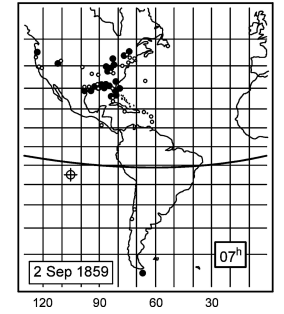
\includegraphics[scale=1]{carrington-spatial.png}
    \caption{{\bf Spatial extent of Carrington Event}: As noted by Cliver and Svalgaard (2004) the Carrington event was observed to very low latitudes in the Americas. Closed circles represent overhead aurora; open circles represent visible aurora. The heavy curved line denotes the geomagnetic equator and the $\bigoplus$ symbol indicates the anti-Sun point. The lowest geomagnetic latitude at which the storm was observed was Honolulu (not shown).}
    \label{fig:carrington-spatial}
 \end{center}
\end{figure}

On March 13th, 1989, another geomagnetic storm, less than a third of the strength of the 1859 Carrington event, disrupted power in Canada and the United States, resulting in blackouts for the majority of Quebec for nine hours; the cost for repair was \$6 billion \cite{cervantes:2013a}. A much smaller event occurred in 2003, known now as the Halloween event \cite{muller:2014, viljanen:2014}. In preparation, satellites were placed into a stable stand-by mode. Ultimately, only one satellite was damaged with most satellites unscathed and exceeding their nominal lifespan. An extreme Carrington event was observed pointed away from Earth in 2012 \cite{eastwood:2017}. It is difficult to quantify the total cost; estimates of the damage a modern Carrington event would cause range from \$140 billion to \$3.4 trillion \cite{eastwood:2017}.

There are many much more frequent but less devastating solar events, discussed in Section \ref{sec:space-weather-events} that can cause damage to power grids, satellites, Earth communications, astronauts, and many other sensitive systems. While they cannot be prevented, advanced warning allows for preparation that can mitigate the damage. Coronal mass ejections, one danger resulting when the Sun spews large amounts of charged material sometimes towards Earth, have been recorded to reach speeds of up to 2000 miles per hour, reaching Earth within the day \cite{fastcme}. Within minutes to hours of a solar flare, the ionospheric disturbance can interrupt radio communications \cite{swap}. For proper safety protocols to be enacted, fast warning of an event is necessary.  This thesis explores solar feature classification through modern machine learning approaches, specifically the creation of a computer vision systems utilizing satellite imagery to identify solar activity in real time for quick response. These classification systems allow for real-time warning of space weather events.

\section{Goals}

This thesis has several key goals as outlined here:
\begin{itemize}
\item There does not exist a curated database of human annotated solar images. This thesis will present the first of its kind, comparing it to existing automated databases. In addition, this thesis will analyze the human labeling to understand agreement/disagreement between different annotators and consistency for each annotator. In order to create this database, the necessary labeling software will be created in this thesis.
\item This thesis will provide a suite of modern machine learning approaches to solar image classification with a random forest, Bayesian, and neural network implementation. These will be compared to existing solar classification approaches as well as each other to characterize their strengths, weaknesses, and overall performance.
\item Ultimately, high-quality solar image classification opens up avenues of research for solar physics. Thus, a prototype solar feature database will compiled from the images, indexing the images and allowing solar physicists to easily find interesting events. Further, a research application estimating the fractal dimension of active regions and properties of coronal hole will be presented.
\end{itemize}

\section{Organization}
Chapter \ref{ch:background} introduces the background information for solar physics in Section \ref{sec:solphys} and machine learning \ref{sec:ml}. This includes a definition of the relevant solar structures to classify.  Then, Chapter \ref{ch:relatedwork} documents prior work in solar imge classification including both the unsupervised systems in Section \ref{sec:unsupervised} and superverised systems in Section \ref{sec:supervised}. The author's original contributions begin in Chapter \ref{ch:data}, after a description of the solar imagery, with an overview and analysis of the human annotated images. Chapter \ref{ch:classifiers} details the classifiers tested in this approach through experiments in Chapter \ref{ch:experiments}. Two applications of the solar classification are explored in Chapter \ref{ch:application}: the labeled solar database in Section \ref{sec:database} and fractal dimension estimastion for solar features in Section \ref{sec:fractal}. Finally, Chapter \ref{ch:conclusion} outlines the results of the entire project and potential future work. 

\chapter{Background} \label{ch:background}

This chapter describes the background of solar weather as well as an introduction to machine learning used in this project.  

\section{Solar Physics} \label{sec:solphys}

Space weather has dangerous and expensive consequences including harm to astronauts and satellites, destruction of power grids, and routine rerouting of intercontinental flights over the north pole. Coronal mass ejections, one danger resulting when the Sun spews large amounts of charged material sometimes towards Earth, have been recorded to reach speeds of up to 2000 miles per hour, reaching Earth within the day \cite{fastcme}. It is critical to have early warning of such events to enact proper protections. The new Solar Ultraviolet Imager (SUVI), a camera aboard the National Oceanic and Atmospheric Administration's (NOAA) GOES-R weather satellite, responds to this need as it captures an image of the Sun every 10 seconds \cite{suvibg}. This flood of data cannot be digested by human forecasters quick enough, necessitating machine learning image classification to identify important events. Machine learning also allows for organized archival of the projected 20 years of imaging, allowing researchers to find relevant data to test new solar models. This is an interesting supervised machine learning problem because it operates on movies of multi-spectral, noisy images. SUVI by no means is the first satellite to explore this problem. This paper explores existing approaches to the astronomical problem as well as looking at parallel solutions in Earth remote sensing applications. Finally, it explores state-of-the-art computer vision research and new approaches to image segmentation and classification.

Space weather has dangerous and expensive consequences including harm to astronauts and satellites, destruction of power grids, and routine rerouting of intercontinental flights over the north pole. Coronal mass ejections, one danger resulting when the Sun spews large amounts of charged material sometimes towards Earth, have been recorded to reach speeds of up to 2000 miles per hour, reaching Earth within the day \cite{fastcme}. It is critical to have early warning of such events to enact proper protections. The new Solar Ultraviolet Imager (SUVI), a camera aboard the National Oceanic and Atmospheric Administration's (NOAA) GOES-R weather satellite, responds to this need as it captures an image of the Sun every 10 seconds \cite{suvibg}. This flood of data cannot be digested by human forecasters quick enough, necessitating machine learning image classification to identify important events. Machine learning also allows for organized archival of the projected 20 years of imaging, allowing researchers to find relevant data to test new solar models. This is an interesting supervised machine learning problem because it operates on movies of multi-spectral, noisy images. SUVI by no means is the first satellite to explore this problem. This paper explores existing approaches to the astronomical problem as well as looking at parallel solutions in Earth remote sensing applications. Finally, it explores state-of-the-art computer vision research and new approaches to image segmentation and classification.


\begin{table}[ht!]
\centering
 \begin{tabular}{||c m{0.5\textwidth}||} 
 \hline
 Name & Description \\
   \hline\hline
   Active regions & Complexes of brighter and darker regions in UV observations caused by the solar magnetic field piercing through the solar atmosphere \\ \hline \\
   Filaments & A suspension of material high in the solar atmosphere by magnetic arches\\ \hline \\
   Prominences & A filament observed off the disk of the Sun \\ \hline \\
   Coronal holes & Regions where the magnetic field is open with no clear reconnection back into the Sun which allow fast outflow of material \\ \hline \\
   Flares & A sudden brightening on the Sun \\ \hline \\
   Coronal mass ejection & An event when the Sun dispels mass and charged particles, sometimes towards Earth \\ \hline \\
   Sigmoids & S-shaped structures on the surface of the Sun thought to be precursors to flares \\ \hline \\
   Quiet corona & Parts of the Sun devoid of activity \\ 
 \hline
 \end{tabular}
 \caption{Solar phenomena: This is a short description of some of the solar events related to space weather. }
 \label{tab:solarfeatures}
\end{table}


Earth is situated inside the Sun's tremendous magnetic field. Features on the Sun evolve and expose Earth to new environmental conditions. The interaction between the Sun's magnetic field and Earth is called space weather.

\subsection{Solar Structures}

\subsection{Space Weather Phenomenon} \label{sec:space-weather-events}

\subsection{Space Weather Mitigation}

\section{Machine Learning} \label{sec:ml}

\subsection{Machine Learning Experiment Design}

\subsection{Classifiers}

\subsection{Computer Vision}

\chapter{Related work} \label{ch:relatedwork}
\section{Synoptic Charts and Thematic Maps}
When classifying space weather phenomena, it is important to understand its context: where it is on the solar disk, when it developed, and its strength. The Sun has a consistent radial outflow of material at approximately 400 km/s as it rotates on its axis every 25 days. This results in magentic field lines in a spiral pattern called the ``Parker Spiral.'' As such, an ejection of material from the Sun on the eastern side of the Sun will reach Earth quicker than an ejection from the western side of the Sun.  Thus, knowing the both the location of the event and the time of the event is very important when considering when the impacts will be felt on Earth. A detailed understanding of the strength of the event and exigent conditions is required to estimate the impact on Earth when it does arrive.

The necessary information can be summarized in a solar synoptic chart. Solar synoptic charts (also referred to as solar thematic maps) detail the solar activity at any given moment using a labeled image of the Sun. While not reponsible for synoptic maps' invention Song et al. (2015)  describe the necessary components of synoptic charts \cite{song:2015}. The synoptic chart must be produced in real-time so that space weather forecasters can read and respond as needed. It must be quantitative when describing observations and object boundaries so that the information can be used in other follow-up systems such as expert validation and database generation. Finally, it must be comprehensive, providing more than sufficient information and easy to examine images of the Sun at various important solar atmospheric heights and temperatures. Based upon a literature study, Song et al. (2015) argued that magnetogram and extreme ultraviolet (EUV) imagery are most valuable for general solar event classification \cite{song:2015}. They created a database of 1586 space weather papers and investigated which types of solar phenomena are correlated to different wavelengths in modern research. After analyzing these trends for active regions, coronal holes, filaments/prominences, flares, and coronal mass ejections, they found that for all the categories 87.4 \% used magnetograms and 59 \% used extreme ultraviolet images. Thus, these two types of data should be featured most prominently on any synoptic charts.

At the moment, reliable synoptic charts used in forecasting are predominantly human drawn. There are existing automatic classifiers, but they often only detail one type of feature. Space weather forecasters at NOOA's Space Weather Prediction Center (SWPC) still hand draw synoptic maps daily, outlining magnetic field lines, coronal holes, flares, filaments/prominences, and plages. Historical maps are \href{http://www.swpc.noaa.gov/products/solar-synoptic-map}{available in PDF format} back until 1972. In a future project, this could serve as an interesting source of labeled data, especially for the difficult task of finding magnetic neutral lines. Zheng et al. (2016) utilized similar synoptic drawings from Yunnan Observatory to extract text annotations about sunspots with a convolutional neural network \cite{zheng:2016}. Some observatories are moving toward automated feature classification. For example, when the person in charge of synoptic maps at the Meudon Observatory was set to retire, they implemented a filament classifier and tracker \cite{meudon:2007}. 

\begin{figure}[ht]
  \begin{center}
    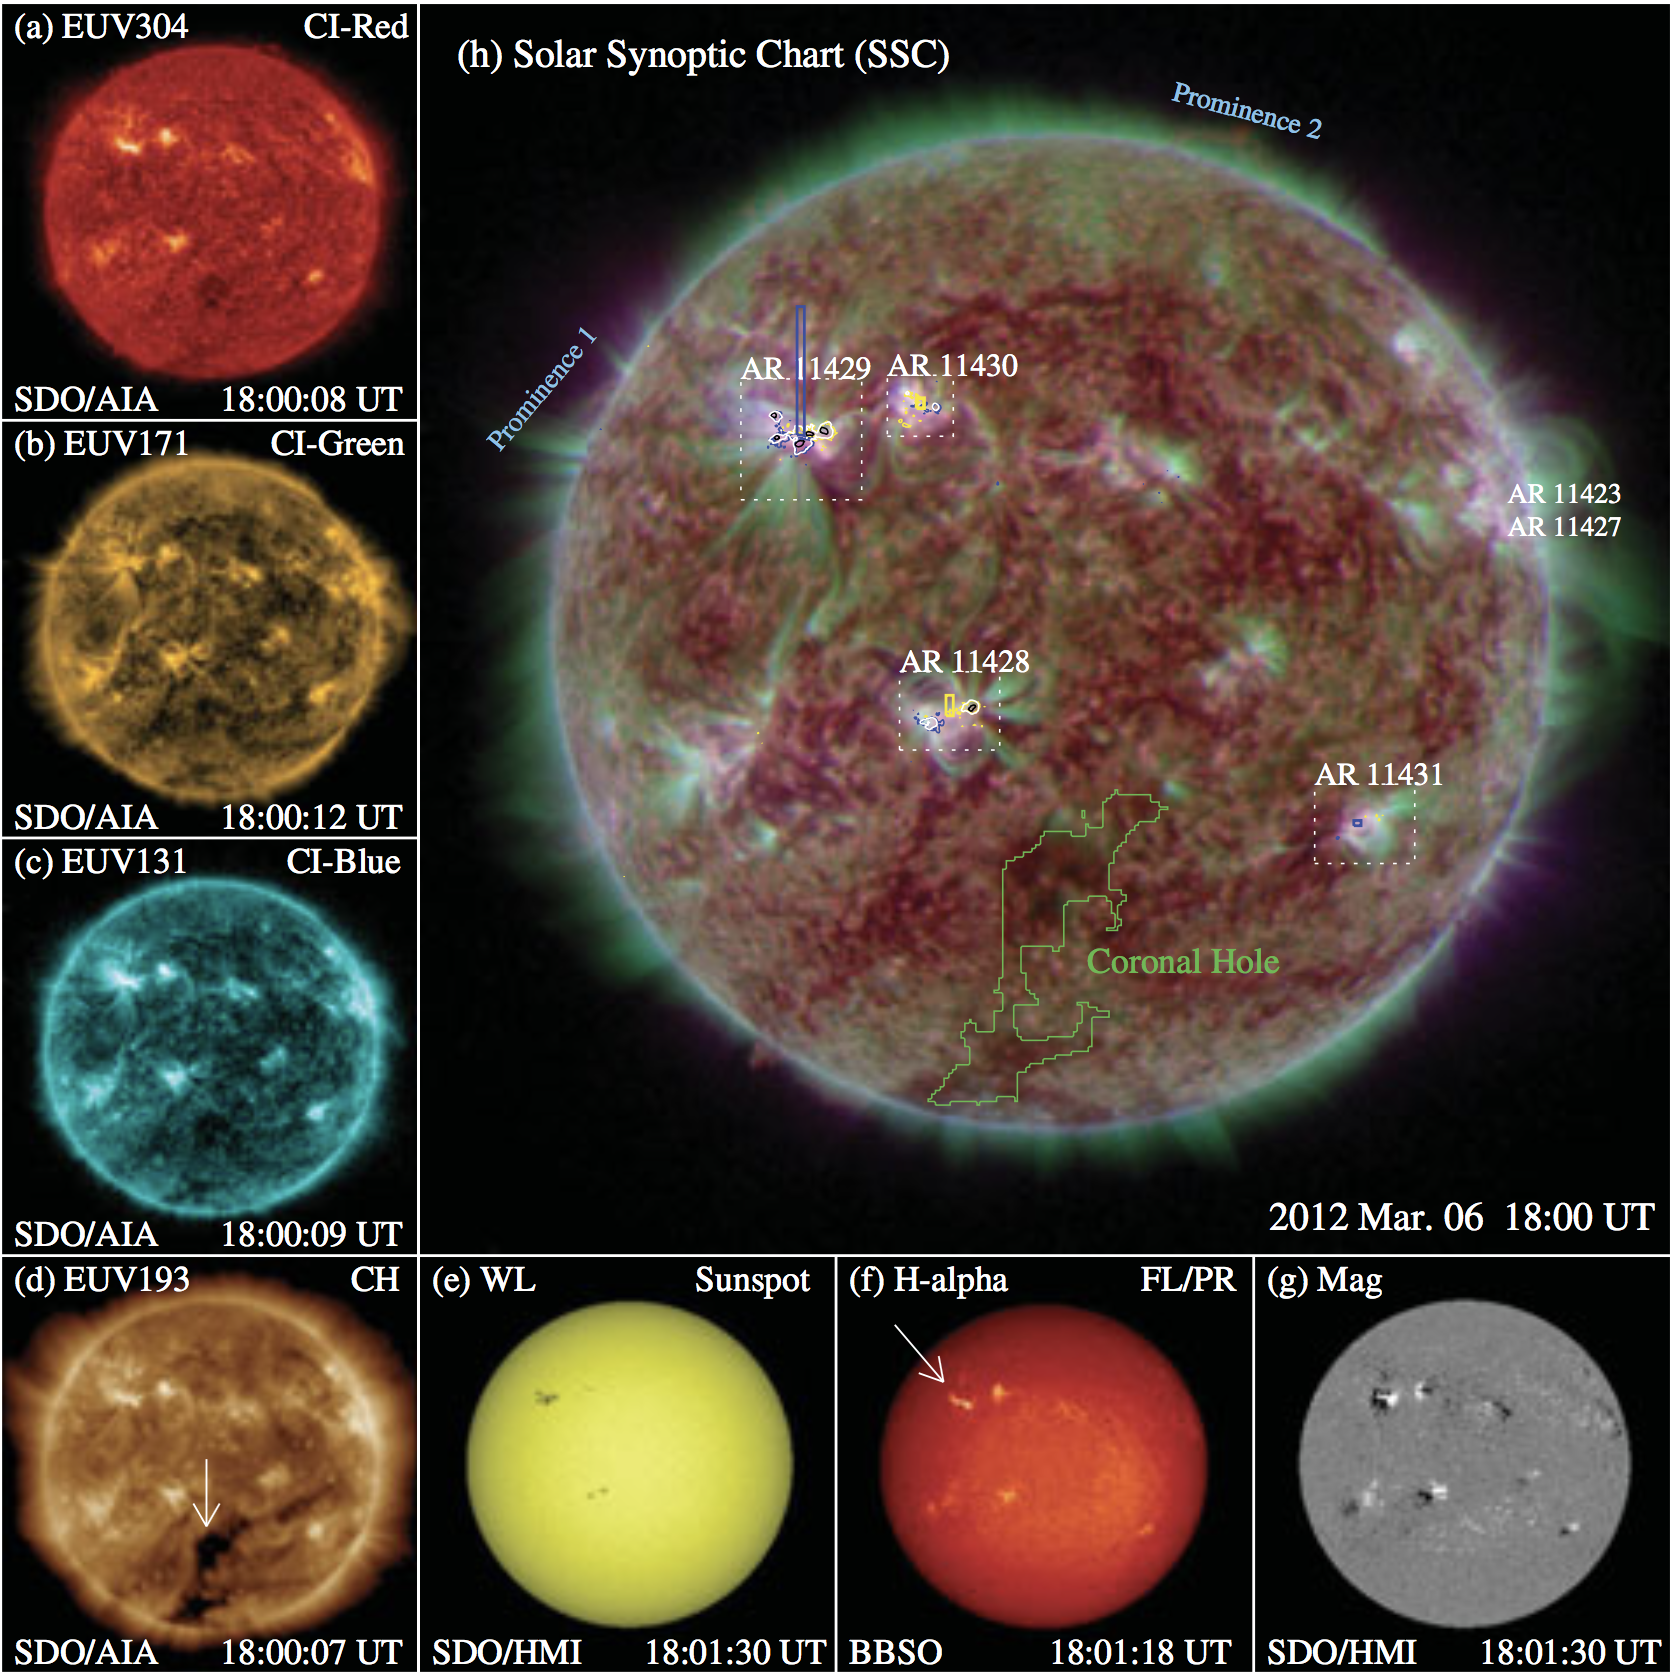
\includegraphics[scale=0.25]{ssc_example-song-2015.png}
    \caption{{\bf Synoptic map example}: Song et al. (2015) propose the solar synoptic map to include a labeled composite image with different wavelength images accompanying to provide a full image of solar activity \cite{song:2015}. }
    \label{fig:sccexample}
 \end{center}
\end{figure}

\section{Data sources}
\subsection{Raw imagery to classify} 
For solar image classification many types and sources of images can be utilized. While brand new imagers like the Solar Ultraviolet Imager (SUVI) do not yet have public data repositories, Sunpy, a python package for solar physics, provides an interface for the Virtual Solar Observatory's large database of solar images \cite{sunpy}. Unsupervised approaches to the problem use this tool and others like it to fetch H$\alpha$, ultraviolet, x-ray, white light, magnetic, and other forms of solar images. They utilize from the Solar Dynamics Observatory, the Solar and Heliospheric Observatory, Solar Terrestrial Relations Observatory, Transition Region And Coronal Explorer, the Global Oscillation Network Group, and many other sources. There is continuous imagery of the Sun at many wavelengths and heights; raw data is generally not a limitation. Instead, the limitation is incorporating raw imagery into a classifier or obtaining labeled data for a supervised trainer. 

\subsection{Labeled data for training} 
The supervised techniques discussed in Section \ref{sec:supervised} require labeled data to train their classifiers. A research group formerly at Montana State University and now at Georgia State University has collated large amounts of images with labeling from unsupervised classifiers. The original dataset in 2013 comprised over 15,000 images with 24,000 events observed in the first half of 2012 by the Solar Dynamics Observatory (SDO). Using the SDO unsupervised classifiers, small grid regions of the image were labeled active region, coronal hole, filament, flare, sigmoid, and sunspot. Each grid region is also statistically analyzed and assigned an entropy, mean, standard deviation, fractal dimension, skewness, kurtosis, uniformity, relative smoothness, contrast, and directionality measures \cite{schuh:2013}. This data was later incorporated into a database tool that allows the user to identify an example image and query the full dataset for similar events \cite{banda:2014}. This dataset and tool was later expanded to the full SDO observing database \cite{schuh:2016}. 

\section{Solar machine learning}
Solar machine learning can be divided into two categories: unsupervised and supervised. Unsupervised techniques do not required human input of labeled images but instead often run on rules; this approach is much more common in astronomy. Supervised techniques are often more flexible and outperform unsupervised techniques in other related fields \cite{anzanello:2014, yu:2013,guerra:2011, huang:2017}. Due to the lack of consistent evaluation, one cannot directly claim this for solar segmentation.

\subsection{Unsupervised solar segmentation} \label{sec:unsupervised}
Unsupervised solar segmentation can be broken into many approaches: edge-based algorithms, region-based algorithms, hybrid algorithms, and artificial intelligence approaches. The first three categories are more image-processing techniques solely while artificial intelligence approaches are more generic examples of clustering, support-vector machines, and other tools. These can be used in tandem with the pure image processing techniques. 

\subsubsection{Edge-based algorithms}
Edge-based techniques utilize discontinuities and identify different features utilizing boundaries. Curto, Blanca, \& Martinez (2008) employed edge-based unsupervised detection when identifying sunpots in H$\alpha$ images \cite{curto2008automatic}. Since sunpots have crisp boundaries their edges can be used to quickly identify them. Curto, Blanca, \& Martinez (2008) used morphological operations to emphasize these boundaries: erosion, dilation, opening, closing, and the top hat transformation. Erosion shrinks bright regions by removing boundary pixels while dilation grows them. Dilation will also fill holes in features. Opening is an erosion followed by a dilation while closing is dilation followed by erosion. Both closing and opening smooth the image: opening fills shape holes, whereas closing breaks wide lines and erases thin lines \cite{curto2008automatic}. The top hat transformation subtracts the original image by the closing of the image. It results in an image showing only the erased parts. By stringing together an empirically determined set of operations, they were able to reliably identify sunpots. Qu et al.(2005) ave a similar system that identifies filaments \cite{qu2005automatic}. 

\subsubsection{Region-based methods}
Region based approaches include histogram segmentations, clustering/thresholding, and region-growing approaches. Fuller, Aboudarham, and Bentley (2005) implemented a filament classifier using region growing \cite{fuller:2005}. This work is based off more generic computer vision region growing by Gonzalez \& Woods (2002) \cite{gonzalez:2002}. After calibrating, removing dust, and sharpening the solar H$\alpha$ images \cite{standardization}, seed pixels are chosen for region growing using a thresholding technique. Only the dimmest pixels are chosen since they should be at the center of filaments. For multiple iterations, the region grows adding new pixels that are connected to seeds and follow the mean and standard deviation of the neighborhood and consequently are similar to the seed. Finally, a morphological closing operation is applied to remove any holes and make the filaments smoother. After this, the center line of the filament can be determined and characterized using a combination of convolutions, dilations, and erosions. This characterization makes it easier to track filament evolution and measure their length. Ultimately, this technique produced 1149 filaments compared to a human labeled 1232 filaments \cite{fuller:2005}. This resulted in missing 10\% of the filaments in an image. Roughly 5\% of the detections were false positives, keying on sunspots instead of filaments because there was no spatial requirement for filaments to be long and skinny. Thus, they could be confused for sunspots which are also dark in H$\alpha$ images. Other region growing methods include: Benkhalil et al.(2006) which used ionized calcium, H$\alpha$, and extreme ultraviolet imagery to grow active region boundaries \cite{benkhalil}, Higgins et al. (2011) which combined magnetograms, image differencing, and region growing to identify and track emerging active regions \cite{higgins}, and McAteer et al. (2005) which used full-disk magnetograms to identify magnetically significant regions and characterize their flare potential \cite{mcateer}. 

Instead of growing regions, one can identify significant features by looking at the histogram of their intensities in various wavelengths. Olmedo et al. (2008) designed such a system to identify coronal mass ejections. The intensity in solar images can be plotted as a histogram as a function of position angle as shown in Figure \ref{fig:olmedo}. A threshold is used to determine what is a significant event in the histogram. If portions of the histogram exceed this, they are declared a region in the image and grouped together. Some region growing is also used in this approach. Ultimately, they were able to recover about 75\% of the human identified coronal mass ejections in a 12-month period. Interestingly, they found an equal number of small coronal events that had been overlooked by humans, often weaker but creating an interesting new population for scientific research and space weather awareness \cite{olmedo2008automatic}. 

\begin{figure}[ht]
  \begin{center}
    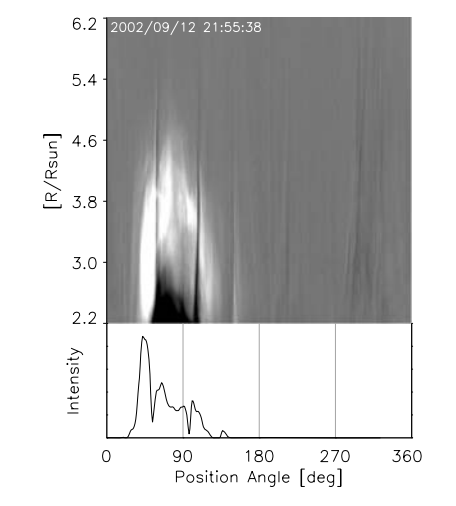
\includegraphics[scale=1]{olmedo.png}
    \caption{{\bf Histogram segmentation}: Olmedo et al.(2008) utilized histogram segmentation to identify coronal mass ejections. ``The intensity profile along the angular axis showing the 1D projection of the CME image. Only positive pixels along the radial axis are used. This profile effectively indicates the angular positions of a CME when it is present.'' \cite{olmedo2008automatic}}
    \label{fig:olmedo}
 \end{center}
\end{figure}


Other histogram based methods include Preminger et al.(2001) which used contrast ratios between ionized calcium and magnetograms to identify sunspots and faculae \cite{preminger}.

\subsubsection{Hybrid}
Some approaches bridge between region-based and edge-based techinques. One key example is SPoCA, a fuzzy classifier that uses multiwavelength extreme ultraviolet observations to assign multiple classes: quiet Sun, active region, and coronal hole. SPoCA is more accurately a suite that implements three types of fuzzy clustering algorithms tailored to the segmentation of solar coronal EUV images: Fuzzy C-means (FCM),  Possibilistic C-means (PCM) algorithm, and Spatial Possibilistic Clustering Algorithm (SPoCA) \cite{verbeeck2014spoca}. It differentiates itself from other techniques because of its reliance on fuzzy logic. Barra et al. (2008) note that the use of fuzzy logic allows the algorithm to overcome noise in the images and the scientific definitions of solar features while meeting many needs. Often, unsupervised solar segmentation techniques are developed with a specific research question and thus are very restricted. For example, one classifier may focus only on the brightest cores of active regions to study energy transfer while another may be designed to catch active regions as they form and thus catch many weak active regions. SPoCA is generic enough to overcome this conflict.

SPoCA works by utilizing the assumptions of fuzzy logic. Each pixel has membership in all of the different classes used in the thematic map. The sum of all the memberships for a pixel must be one, i.e. the pixel membership indicates how much the pixel matches that theme. In fuzzy c-means \cite{cmeans}, a generalization of K-means clustering to fuzzy logic, the variance within a cluster, all the pixels labeled a theme, is minimized. This approaches is very susceptible to the noise in astronomical images though \cite{krishnapuram1993possibilistic}. Thus, the fuzzy c-means requirement of membership summing to one is relaxed to form of possibilistic c-means \cite{krishnapuram1996possibilistic}. SPoCA is a further modification that incorporates weighting by spatial extent such that neighboring pixels should be assigned similar labels \cite{barra:2008, barra:2009}. 

Barra et al. (2009) used SPoCA to both segment and track features on the Sun \cite{barra:2009}. They exercised the power of SPoCA to perform two very different experiments. First, they tracked the biggest active region for a month, quantifying its size, average intensity, fractal dimension, and other parameters for scientific inquiry. Then, they identified and tracked coronal bright points, a feature not initially intended in SPoCA. These short lived ($< 2$ days) bright regions have some spectral similarity to active regions but are much smaller and can appear within coronal holes. They impact the structure and dynamics of the solar corona. During the study, Barra et al. (2009) tracked their counts, north/south asymmetry, intensity fluctuations, and other parameters \cite{barra:2009}.  

There are other types of unsupervised classifiers that do not fit nicely into the two main categories. For example, Bratsolis \& Sigelle (1998) utilized mean field fast annealing to segment sunspots \cite{bratsolis1998solar}. The approach uses simulated annealing to minimize the classification into $q$ classes. Each pixel is assigned a label. This labeling has an energy described by mean field theory and the Potts interaction between pixels. Essentially, this approach attempts to find the most meaningful classification. It excels over histogram methods which often are not granular enough to separate regions of different activity in the sunspot.

\subsubsection{Example system: Solar Dynamics Observatory}
Many unsupervised approaches that only deal with one class at a time can be chained together to create all the necessary data for a thematic map. The Solar Dynamics Observatory (SDO) satellite mission produces 1.5 TB of imagery per day in multiple ultraviolet wavelengths, a magnetogram, and other data channels. To deal with this influx of data, teams of researchers developed classifiers that identified specific classes of features \cite{sdo}. All of the component parts can be seen in Figures \ref{fig:sdo1} and \ref{fig:sdo2}.

\begin{figure}[ht]
  \begin{center}
    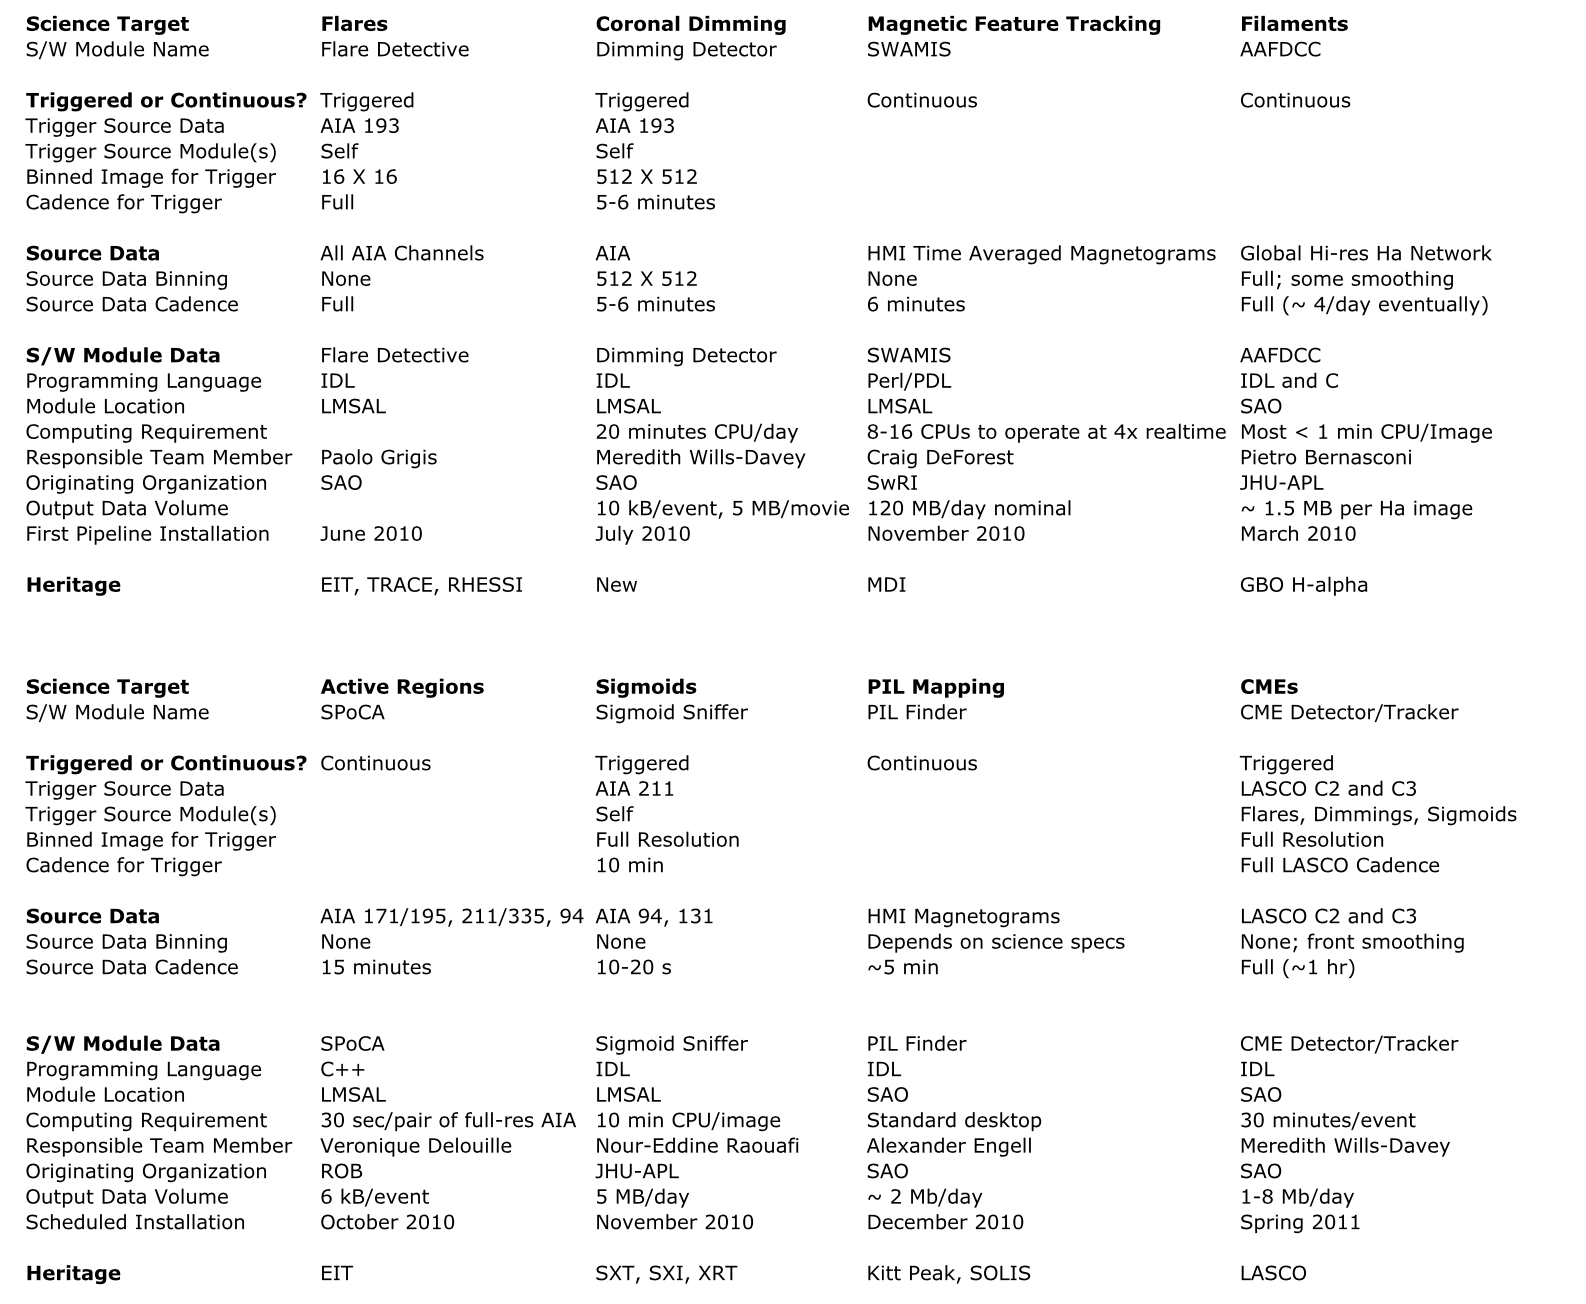
\includegraphics[scale=0.5]{sdo1.png}
    \caption{{\bf First half of SDO classifiers} \cite{sdo}}
    \label{fig:sdo1}
 \end{center}
\end{figure}

\begin{figure}[ht]
  \begin{center}
    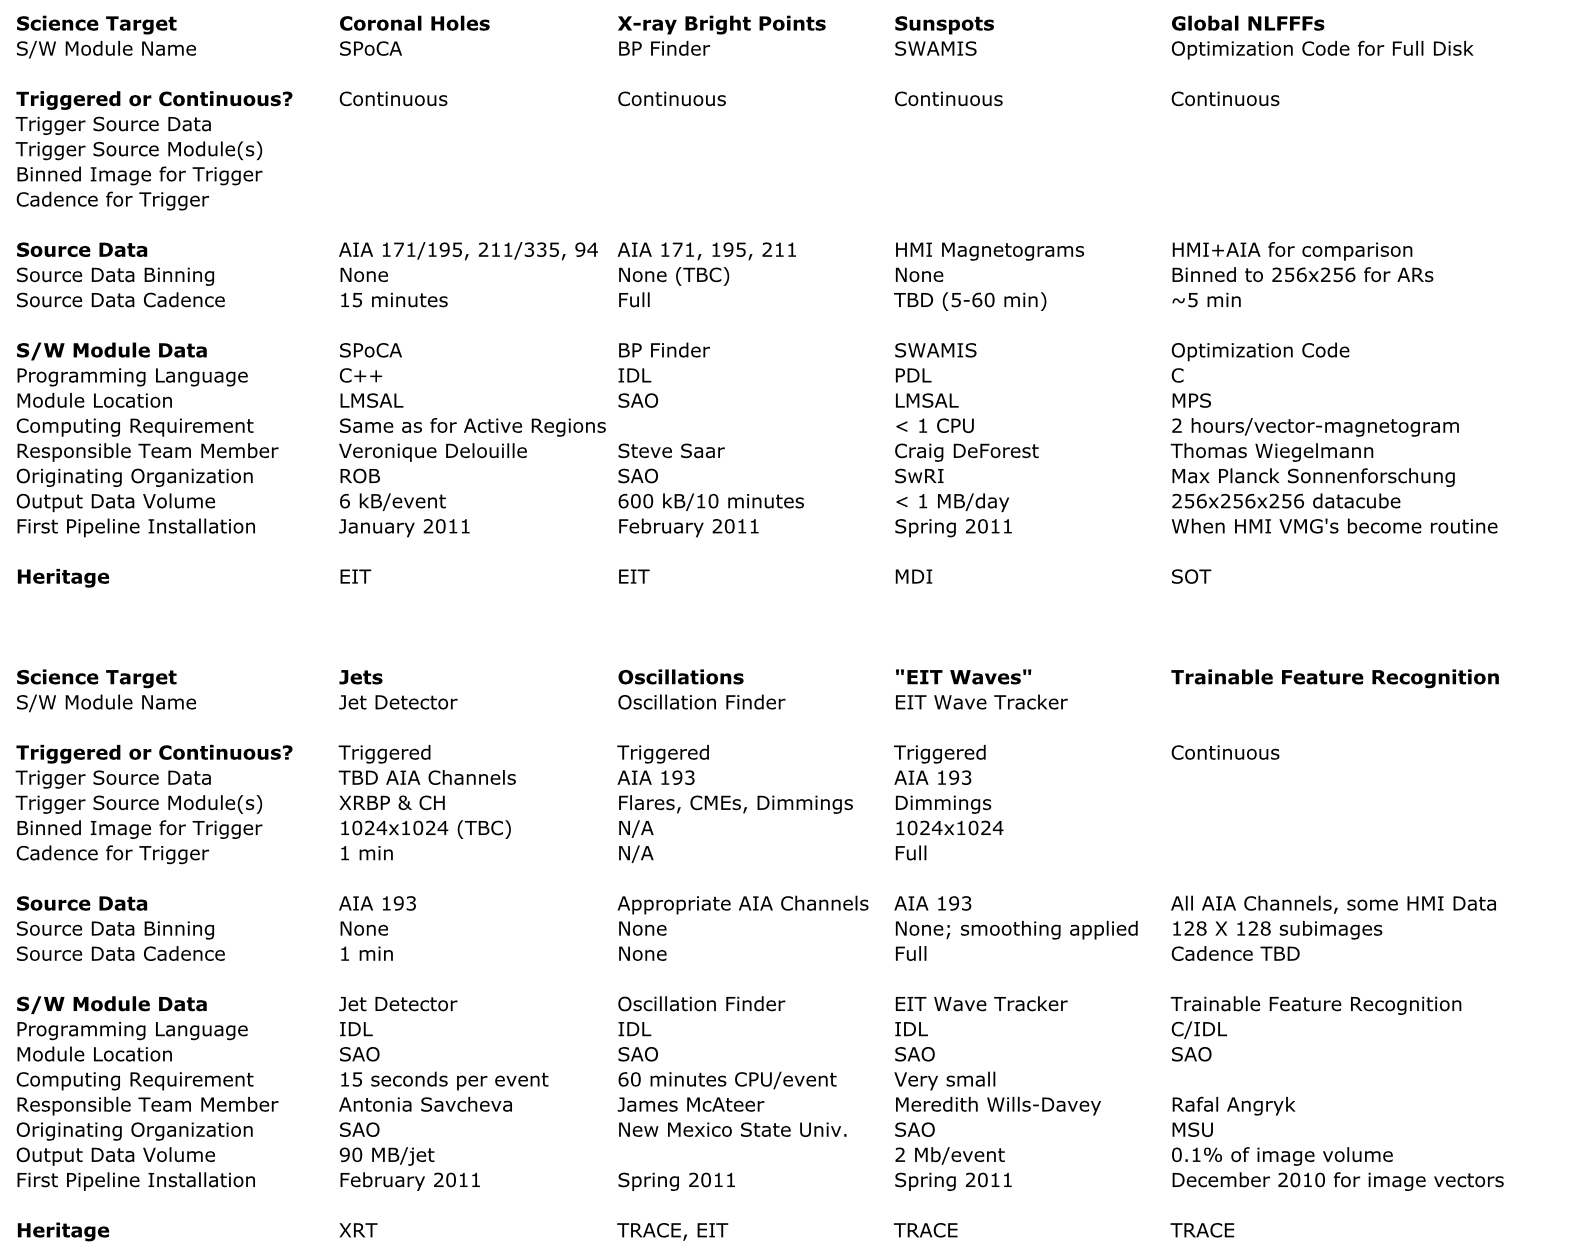
\includegraphics[scale=0.5]{sdo2.png}
    \caption{{\bf Second half of SDO classifiers} \cite{sdo}}
    \label{fig:sdo2}
 \end{center}
\end{figure}

The SDO suite suite is a comprehensive approach to classification that utilizes all of the techniques mentioned thus far and more. For features that are beyond the individual classifiers' scope, a trainable module is employed. While this is a supervised system, it is mentioned here to emphasize the difference between supervised and unsupervised approaches. A user can identify a specific type of feature they are interested in by identifing them within an image. These are placed in feature vectors of 12 texture paramters (e.g. mean, entropy, uniformity). These train either a support vector machine or a C4.5 decision tree and will then identify similar features from the rest of the database \cite{lamb2008example}. The SDO suite lacks the ability to combine all the classifications into a single thematic map. 

\subsubsection{Comparisons}
\begin{figure}[ht]
  \begin{center}
    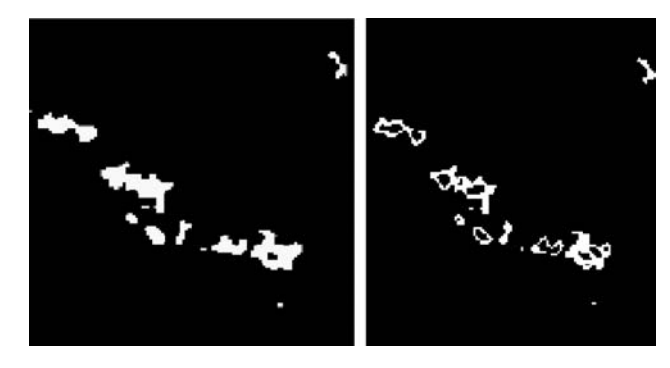
\includegraphics[scale=1]{revathy.png}
    \caption{{\bf Performance of different methods}: Revathy, Lekshmi, \& Nayar (2005) compared the performance of different segmentation techniques in identifying active regions \cite{revathy}. At left is the result of a histogram thresholding approach while at the right is fuzzy-based segmentation. }
    \label{fig:revathy}
 \end{center}
\end{figure}

As shown in Figure \ref{fig:revathy}, different methods produce often similar but still different results. By computing the fractal dimension over the segmented image, they were able to characterize the difference between fuzzy clustering, region growing, iterative thresholding, and histogram thresholding. They found that depending on the height of the active region in the solar atmosphere it was segmented differently. In general, the fuzzy-based and histogram approaches outperformed the others. They propose that using longer wavelength ultraviolet images tends to larger area active regions.

Caballero \& Aranda (2013) conducted an independent comparison of unsupervised techniques for active regions \cite{caballero}. Using 6000 images from SOHO in 195 angstroms, they initially segmented the images using region growing techinques. Then, the different independent regions were clustered together into units using either partition approaches or a hierarchial classification. They found that the hiearchial classification, the idea that nearby regions should be more strongly connected, produced more human-like clusters. However, this approach requires exponential time complexity and results in a hierarchy instead of a simple division into clusters.

For a much longer comparison of many different techniques see Aschwanden (2010) \cite{aschwanden:2010}. 

\subsection{Supervised solar segmentation} \label{sec:supervised}
There are relatively few supervised solar segmentation approaches but the existing approaches are very promising and tend to perform on a broader set of classes and image types. Thus, a bit more detail is provided in describing each approach. 

\subsubsection{Maximum likelihood estimation}

Rigler et al. (2012) proposed a preliminary naive Bayesian classifier for SUVI images using the Solar Dyanmics Observatory (SDO) Advanced Imaging Array (AIA) observations for testing \cite{rigler:2012}. Their work focused on eight classes: flare, prominence, active region, quiet corona (off-disk), quiet corona (on-disk), coronal hole (off-disk), coronal hole (on-disk), and outer space. They were able to achieve an average accuracyof 86\%. This was calculated by training the classifier on a set of data then testing it on a classified image that was not used for training. The tabulation was done strictly on a pixel by pixel basis, not checking if the error was coherent or random noise. Prominence was the most problematic class with only 41\% of prominence pixels being classified correctly. They were often misclassified as off-disk quiet corona or on-disk coronal hole.

The naive Bayesian approach works by classifying every pixel into one of $n$ classes using multispectral ultraviolet images. Therefore, a pixel, a spatial element at $(i,j)$ corresponds to $h$ channels and can be described as a vector:
\[ x_{(i,j)} = \begin{bmatrix} x_1 & x_2 & \hdots & x_h \end{bmatrix}^T \]
The approach is assign each $x_{(i,j)}$ pixel a label $w_k$ from the set of classes $W$. This approach employs Bayes' Theorem:
\[ P(w_k | x_{(i,j)}) = \frac{P(x_{(i,j)} | w_k) P(w_k)}{P(x_{(i,j)})} \]
Since $P(x_{(i,j)})$ is not a function of the label classification, it can be ignored.
\[ P(w_j | x_{(i,j)}) \propto P(x_{(i,j)}) P(w_{k}) \].
Rigler et al. (2012) simplify this even further by stating that ``if there is no a priori reason to believe a pixel should be assigned label $w_k$, $P(w_k)$ can be assumed to be drawn from a uniform distribution''. Thus,
\[ P(w_k | x_{(i,j)}) \propto P(x_{(i,j)} | w_k) \]
This approach is the maximum likelihood solution to this problem.

For training they simplify each class into a multivariate normal, i.e. for each potential label there is a archetypal example pixel and all pixels with that label should be distributed normally about it. This is overly constraining if any given class has multiple distinct modes with respect to the selected data. The multivariate distribution for class $w_k$ is characterized by a mean vector $\mu_k$ and covariance matrix $C_k$ which are calculated as:
\[ \mu_k = \frac{\sum_{x \in W_k} x}{|W_k|} \]
where $W_k$ is the collection of pixels with label $w_k$. Similarly,
\[ C_k = \frac{\sum_{x \in W_k} \begin{bmatrix} x - \mu_k \end{bmatrix} \times \begin{bmatrix} x - \mu_k \end{bmatrix}^T}{|W_k|} \].
These mean vectors and covariance matrices characterize the class. Given this characterization for class $w_k$ one can calculate the conditional probability of a pixel $x_{(i,j)}$ having label $w_k$:
\[ P(x_{(i,j)} | w_k) = \frac{1}{\sqrt{(2 \pi)^h} \sqrt{|C_k|}} \mathrm{exp} \left( \frac{-1}{2} \times \left(x_{(i,j)} - \mu_k \right)^T \times C_k^{-1} \times \left(x_{(i,j)} - \mu_k \right) \right) \]
Thus, the pixel is assigned the class that maximizes this probability.

Since each pixel is treated separately, any noise in single pixels or in the image as a whole can result in a noisy classification where a pixel class does not agree with its neighboring pixels as expected. Therefore, Rigler et al.(2012) propose a smoothness prior be enforced so that a pixel's labeling relies on its neighbors This can be enforced by iteratively calculating the thematic map, calculating a smoothed map relying on neighbor probabilities, and repeating until convergence using simulated annealing, maximizing posterior marginals, or iterated conditional modes as proposed by Tso and Mather (2009) \cite{tso:2009}. 

Their results were promising with high accuracies and maps that generally coherent. However, their results are concerning because some statistics and accuracy measurements come from running the classifier on training data, providing no indication on how the classifier would perform on unfamiliar, real-world examples. 

Rigler et al.(2012) built upon earlier work by de Wit (2006) who suggested the Bayesian approach \cite{dewit:2006}. After decreasing the noise and normalizing the intensity in each image, de Wit(2006) instead used only four ultraviolet wavelengths and projected them into a three-dimensional parameter space using singular-value decomposition \cite{dewit:2006}. Thus, de Wit(2006) ran a naive Bayesian classifier on these transformed parameters instead of the higher dimensional wavelengths. Figure \ref{fig:dewit} shows an example result by de Wit(2006), emphasizing the coherence of this segmentation without any forced smoothness \cite{dewit:2006}. This approach ran in near real-time, taking only a few minutes to classify every pixel. 

\begin{figure}[ht]
  \begin{center}
    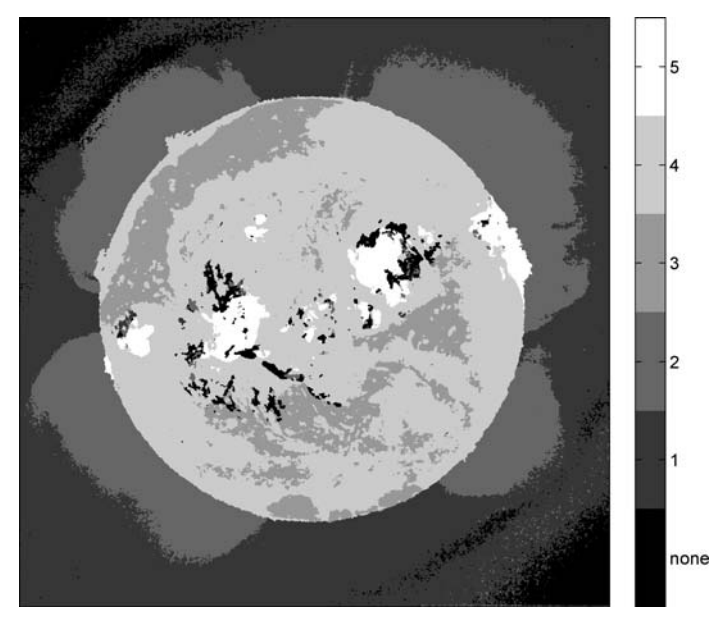
\includegraphics[scale=1]{dewit.png}
    \caption{{\bf de Wit Segmentation}: This figure indicates the power of quick, multi-spectral, supervised segmentation done by de Wit (2006), very similar to other work by Rigler et al.(2012) and Visscher et al.(2015) \cite{dewit:2006}. The classes for this study are: ``(1) Tenuous corona outside of the disk, in regions with open magnetic-field lines.(2) Dense corona outside of the disk. (3) Coronal holes. (4) Quiet sun, including the chromospheric network and regions inside the network boundaries. (5) Active regions on the disk'' \cite{dewit:2006}. }
    \label{fig:dewit}
 \end{center}
\end{figure}

\subsubsection{Maximum A Posteriori}
Visscher et al. (2015) improve upon Rigler et al. (2012)'s result by recognizing that the classes are not equally likely (e.g. the majority of the Sun is covered by quiet corona at any given time) and that crisp segmentation procedures are too limiting compared to fuzzy segmentation \cite{visscher:2015}. Further, they incorporate spatial information by letting the probability of a class rely on both the intensity and latitude, assuming these are statistically independent variables so $p((x, L(x)) | w_k) \approx P(x|w_k) P(L(x)|w_k)$ where $L(x)$ is the latitude of the pixel and $w_k$ is a class. This addresses the observable fact that coronal holes tend to form at solar poles, high latitudes, while active regions form near the equator. Unlike Rigler et al. (2009), Visscher et al. (2015) use only one wavelength of light in their dataset: the 19.3 nm SDO-AIA channel. Additionally, they only assign three classes: active region, coronal hole, and quiet sun. This makes it difficult to directly compare their results because the troubling classes Rigler et al.(2009) observed are not included.  Therefore, the probability they are maximizing is instead: 
\[P(x|w_k)p(L(x) | w_k) p(w_k) \]
While doing this, they have assumed a fuzzy segmentation that allows for degrees of membership in each class. This approach allows estimation of how certain different classes are under different conditions. For example, they confirmed that wrongly classified pixels were classified as half one class and half another class and often on the object boundaries. In adition, they were able to pinpoint that there is disagreement with the gold standard reference. Upon second examination, they find that the human assigned labels may actually be wrong in this region, highlighting a key problem in solar segmentation: there is no clear universally agreed upon definition of some of the classes so no human classification can be accepted as completely correct. Even if a human standard does exist, it is sometimes still impossible to discern between classes due to degeneracy in the observational parameters. Ultimately, they report average 94\% accuracy over all classes.

In addition to accuracy with a single frame, Visscher et al.(2015) establish a criteria for accurate segmentation into large-scale features \cite{visscher:2015}:
\begin{itemize}
\item ``Stable segmentations on short timescales in the absence of major solar activity''
\item Consistent and smooth trends and classifications over longer periods of time
\item Consistency with human drawn maps
\end{itemize}
While there is no quantified method for the first two criteria, they are highly relevant and often not addressed in other approaches explicitly. 

\subsubsection{Neural Networks}
Deep convolutional neural networks have proven to be very skilled in classifying and segmenting in various contexts \cite{szegedy:2015, tso:2009, krizhevsky:2012}. Convolutional neural networks are specifically designed for image data such as solar images. Each layer extracts local features from an image using a kernel which are combined in intermediate pooling layers. This allows for a robust classification with respect to distortions or noise in the images. Activation functions allow only significant features to influence the final classification. Deep learning approaches are advantageous because they automate feature selection by weighting input data according to their training algorithms instead of having a scientist develop detailed rules about what data components indicate which classes.

Kucuk et al.(2017) applied the first convolutional neural network to solar imagery for classification \cite{kucuk:2017}. While classifying over a finer granularity of classes they were able to achieve an average 70\% accuracy across each class. This convolutional neural network approach outperformed the only other published neural network solar segmentation found during this review. Zharkova \& Schetinin (2005) employed a feed-forward neural network with two hidden neurons and one output neuron to identify solar filaments at 82\% accuracy \cite{zharkova:2005}. This result is not directly comparable since it only classified one type of feature. However, it illustrated the power of neural networks in solar images. Filament classification by classical image processing techniques is often confused by the highly variable background between different parts of a filament and from filament to filament. The artificial neural network was able to flexibly learn many patterns and more accurately identify filaments. At the time, it was only outperformed by a region-growing approach \cite{fuller:2005}. 

Up until now, classification has only been discussed in a spatial domain. However, flares and coronal mass ejections have a temporal components. They are by definition changing features. Borda et al. (2002) implemented a simple neural network consisting of two layers (not including input): a hidden layer of nonlinear neurons and
an output layer of one linear neuron \cite{borda2002automatic}. Given optical H$\alpha$ images, it identifies solar flares in real-time. It operates on 7 input features: mean image brightness, standard deviation of the brightness, the pixel of maximum brightness change between images, absolute brightness of pixel with maximum change, radial position of that pixel, variation of mean brightness between two images (to characterize possible weather influences), and the contrast between the pixel with largest change in brightness and its neighbors. Given 124 test events, fewer than 5\% were misidentified. (The paper does not make clear about false positives and false negatives.) Accounting for normal operations, this would be a misclassification every few days. There has been limited solar time series neural networks beyond this, but it establishes a baseline system for future architectures and generalizations to other feature types.

\section{Earth Remote Sensing}
Earth remote sensing of multiwavelength features has many more applications and a longer availability of data and thus has advanced further than solar machine learning techniques. 

This author could not find an example of random forests for solar image classification. However, they are routinely used in Earth remote sensing classifications. Random forests are an ensemble of tree classifiers. To classify a new feature vector, the input vector is classified with each tree in the forest, and the forest chooses the classification having the most votes over all the trees in the forest. Random forests have many advantages: high accuracy compared to current algorithms, efficient implementation on large data
sets, and an easily storable data structure for future use \cite{ghose2010decision}. Lowe \& Kulkarni (2015) used a random forest to identify terrain type in hyperspectral images \cite{lowe:2015}. For this application, the random forest had 96.25 \% accuracy compared to neural network's 76.87\%, support vector machines 86.88\%, and maximum likelihood's 83.11\% \cite{lowe:2015}. This high performance for random forests with this type of problem is not uncommon \cite{puissant2014object, salas2016multispectral, clark2016mapping, kulkarni2017multispectral}.

Similarly, neural networks have a rich tradition in Earth remote sensing. Lee \& Kwon (2017) developed a 9 layer convolutional neural network, both wider and deeper than state-of-the-art methods for this problem, to classify land types in Earth remote sensing \cite{lee2017going}. This network achieves over 95\% accuracy in nearly every class. It is specially designed for spectral-spatial data and explores neighborhood relationships in a more optimized fashion that previous networks by allowing for multi-scale examination.

Li et al. (2014) present a comprehensive review of Earth remote sensing classification techinques based on spatial techniques \cite{li2014review}. They detail the usage of K-means, ISODATA, SOM,
hierarchical clustering, Maximum likelihood, Minimum distance-to-means, Mahalanobis distance, Parallelepiped, k-nearest Neighbors,  artificial neural network, classification tree, random forests, support vector
machine, genetic algorithms, Fuzzy classification, neural networks, regression modeling, regression tree analysis, spectral mixture analysis, fuzzy-spectral mixture analysis,  and image segmentation and object-based image
analysis techniques in Earth remote sensing. 

\section{General Computer Vision}
Cutting edge computer vision research can be applied to the solar segmentation problem. The solar segmentation problem and producing thematic maps is an example of semantic segmentation, a well studied problem in computer vision. 

\subsection{Fully convolutional neural networks}
The notion of extending convolutional neural networks to do dense prediction, effectively creating a thematic map, was first proposed by Matan et al. (1991) \cite{matan} to extend the LeNet convolutional neural network \cite{lenet} for handwritten digit recognition. Shelhamer, Long, \& Darrell (2016) presented a new implementation, the fully convolutional neural network (FCN), that takes arbitrarily sized input and creates a similarly sized semantic segmentation \cite{fcnn}. During their development, they thoroughly describe convolutional neural network for semantic segmentation up until 2016 \cite{fcnn}.

\begin{figure}[ht]
  \begin{center}
    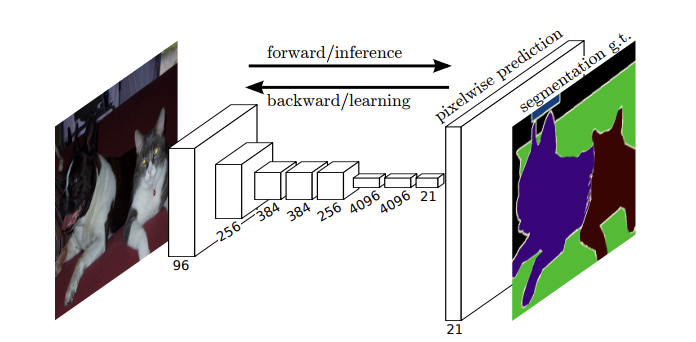
\includegraphics[scale=1]{fcnn.png}
    \caption{{\bf Fully convolutional neural network}: This is an example architecture for a fully convolutional neural network (figure 1 from Shelhamer, Long, \& Darrell (2016) \cite{fcnn}).  }
    \label{fig:fcnn}
 \end{center}
\end{figure}

A FCN works by using existing full neural networks in a convolutional fashion. Then, the last steps of the existing network are removed so that it cannot make a classification for the entire input image at that time. Instead, a pixelwise prediction layer is added using deconvolution and striding over the input image. Without specialized refinement, the FCN can then create a dense output map. At the time, the FCN gave 20\% improvement over state-of-the-art semantic segmentation in a shorter inference time.

\subsection{Mask R-CNN}
He, Gkioxari, Doll{\'{a}}r, \& Girschick developed Mask Regional Convolutional Neural Network (Mask R-CNN), an extension of Faster R-CNN \cite{ren:2017} that creates another form of a semantic segmentation \cite{he:2017}. Technically, Mask R-CNN is a type of FCN \cite{fcnn}. Faster R-CNN worked by quckly determining bounding boxes for various objects in a scene. Mask R-CNN extends this by determining a pixel mask for each bounding box in parallel. Thus, it can distinguish both the type of an object and between neighboring objects in a scene. 

\begin{figure}[ht]
  \begin{center}
    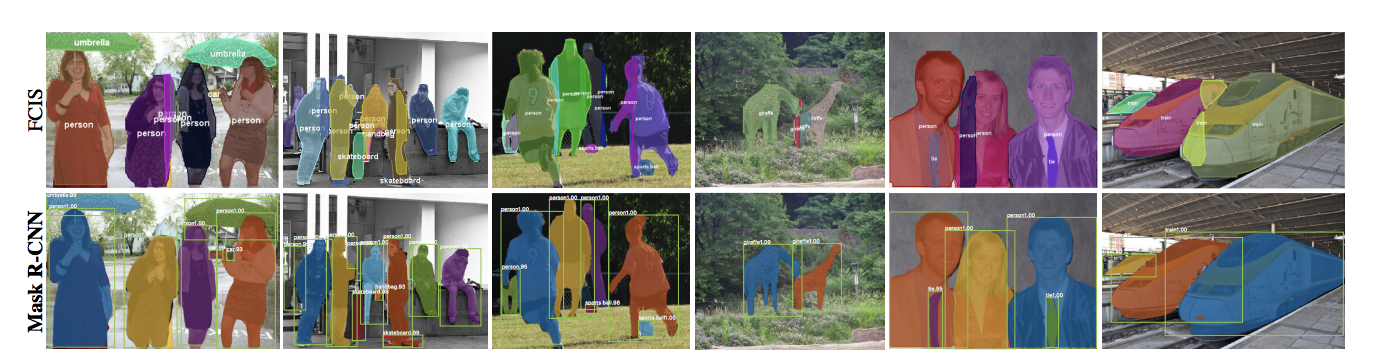
\includegraphics[scale=0.5]{mrcnn.png}
    \caption{{\bf Mask regional convolutional neural networks}: The top row was the existing state-of-the-art instance segmentation \cite{li2016fully}, an example of a FCN, compared to the bottom row of Mask R-CNN performance on the same scene. The overlaid coloration indicates the segmentation while bounding boxes indicate where Mask R-CNN evaluated these masks. Clearlly, the Mask R-CNN produces more coherence classifications. In addition, it runs in less time with higher accuracy than the existing state-of-the-art systems and was consequently awarded the 2017 International Conference on Computer Vision best paper award.}
    \label{fig:mrcnn}
 \end{center}
\end{figure}

The Mask R-CNN design was tested in several domains: cityscapes, human pose estimation, common objects. In all cases, it outperformed existing systems. With modification, this type of architecture solves the problem of solar segmentation. 

\section{Summary}
Solar image segmentation is well motivated by space weather and archival concerns. Up until now, there have been numerous unsupervised approaches, too many to completely document in this paper. These approaches employ a variety of computer vision techniques but are often limited to only determining membership in one class, e.g. determining which pixels are filament. They can be used in tandem to create solar thematic maps that label all classes on the Sun in an ensemble classifier. Settling disputes between the independent classifiers can be difficult and running them all in parallel can be costly. Instead, machine learning techniques can be applied to label the entire image at one time. A few supervised approaches have been developed and perform well. However, there is limited quantification and even more limited consistent quantification of that performance making it difficult to compare systems. By looking to Earth remote sensing and state-of-the-art computer vision machine learning approaches, solar image segmentation can be advanced in a systematic and measurable fashion. 

\chapter{Data} \label{ch:data}

This chapter first describes the raw solar data utilized in this work. It then details the processing done to use the images in the project. Finally, it describes the annotation process for the images and analyzes the results. 

\section{Solar Imagery}
Ultraviolet observations of the Sun are optimal for seeing both dynamic, high temperature solar eruptions and cooler, more stable coronal holes. There are a few ultraviolet solar imagers: the Atmospheric Imaging Assembly (AIA) aboard the \textit{Solar Dynamics Observatory} (SDO) spacecraft \cite{lemen:2012}, the Extreme-ultraviolet Imaging telescope aboard the \textit{Solar and Heliospheric Observatory} (SOHO) spacecraft \cite{eit}, and the Sun Watcher with Active Pixels and Image Processing (SWAP) aboard the \textit{Project for On-Board Autonomy 2} spacecraft \cite{halain:2013, seaton:2013}. This project instead uses data from the new Solar Ultraviolet Imager (SUVI) aboard the \textit{ Geostationary Operational Environmental Satellite 16} (GOES-16) operated by the United States National Oceanic and Atmospheric Administration (NOAA) \cite{suvibg, suvibg2}. SDO, SOHO, and SUVI share many of the same wavelength passbands, but SUVI has a wider field of view allowing for classification of events further off the Sun. SWAP has the same field of view as SUVI but only one passband that SUVI also has. SUVI has a slightly higher spatial resolution than SWAP. In addition, GOES-16 is the first four commissioned satellites in the t-R series, all of which will have SUVI instruments. Thus, the classification system and database built here will be used for at least 20 years. The classification techniques applied here could be applied, with modification, to any of the aforementioned satellites, including to archived data. 

\subsection{Solar Ultraviolet Imager (SUVI) Data}
SUVI observes in six different wavelength passbands (and their corresponding coronal EUV emission line) using filters and multilayer mirrors sensitive to specfic wavelengths: 9.4 nm (Fe XVIII), 13.1 nm (Fe XXI), 17.1 nm (Fe IX/X), 19.5 nm, (Fe XII), 28.4 nm (Fe XV), and 30.4 nm (He II) Each wavelength is most sensitive to a specific wavelength and solar feature as detailed in Figure \ref{fig:suviwavelength}. This is qualitatively apparent in the first-light images from SUVi in Figure \ref{fig:suviimages}.

\begin{figure}[ht]
  \begin{center}
    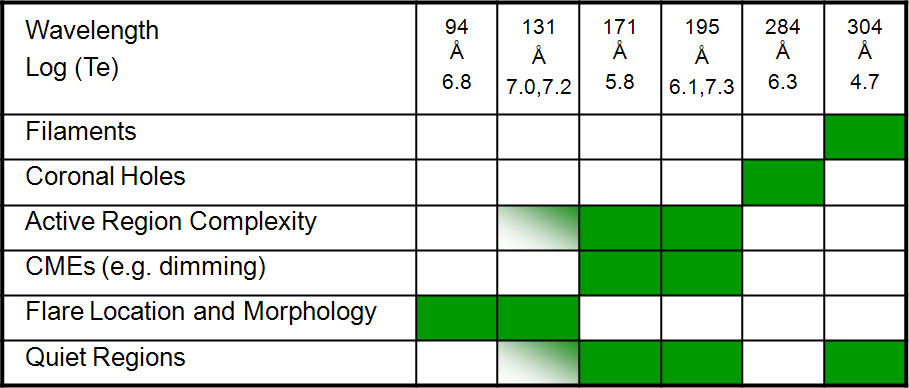
\includegraphics[scale=0.4]{suvi-wavelength-log.jpg}
    \caption{{\bf Wavelengths}: This diagram indicates which SUVI wavelengths are most helpful in identifying different space weather events \cite{suviwebsite}.}
    \label{fig:suviwavelength}
 \end{center}
\end{figure}


\begin{figure}[ht]
  \begin{center}
    \includegraphics[scale=0.8]{suvi-images.jpg}
    \caption{{\bf Example SUVI images}: These first-light images taken on January 29, 2017 exemplify SUVI's response to different solar features in different passbands. For example, the large coronal hole (the darker boot-like shape in the lower portion of the Sun) has higher contrast from the background in 19.5 nm than 304 nm \cite{suviwebsite}.}
    \label{fig:suviimages}
 \end{center}
\end{figure}


Each image is composed of 1280x1280 14-bit pixels. The individual pixels are 2.5x2.5 arcseconds on a side resulting in a 53.3 arcminute total field of view horizontally \cite{suvibg2}. The field of view is slightly larger along the diagonal but vignetting in some of the image corners in some passbands renders these regions unusable. Ultimately, SUVI can observe out to 1.6-2.3 solar radii (depending whether on the horizontal or diagonal). 

One image, in a single passband, is taken every 10 seconds. The observation sequence insures that every passband is observed at least once every four minutes. In addition, SUVI captures a short exposure time and a long exposure time image in each passband. During energetic and bright events like flares, the detector would saturate at the longer exposure time needed for high contrast images during times without energetic events. These two exposure times are combined to create high-dynamic-range composite images, which a two to three orders of magnitude increased dyanmic range than a single exposure time. In addition, SUVI has anti-blooming circuitry so that saturation in the long exposure image does not deteriorate quality in the composite image. This compositing will allow more classification of very bright active regions and flares than if another data set were used. Finally, the composite images are aligned so that the Sun is centered in each. 
\todo{this is all from suvibg2 but how many times should I cite?}

\subsection*{\halpha imagery} 
As discussed in Section \ref{sec:halphainclusion}

\section{Labeled Imagery} \label{sec:labeling}
Since this study is using supervised machine learning, labeled images of the Sun are needed. There does not exist a verified sample of human labeled solar events for more than one category of event. The closest system is the Heliophysics Event Knowledgebase (HEK) \cite{hurlburt:2012} which combines data mining and computer vision with data visualization techniques to create a database of labeled events. These are sometimes verified by humans but can be problematic, especially with multiple entries per event to sift through. Each event is given one of their designated labels as shown in Table \ref{tab:heklabels}.  

\begin{table}[ht!]
  \centering
  \begin{tabular}{||p{4cm} p{10cm}||}
    \hline
    Event Class & Description \\
    Active Region & Solar Active Region\\
    Coronal Mass Ejection & Ejection of material from the solar corona \\
    Coronal Dimming & A large-scale reduction in EUV emission \\
    Coronal Jet & A jet-like object observed in the low corona \\
    Coronal Wave & EIT or Morton waves spanning a large fraction of the solar disk \\
    Emerging Flux & Regions of new magnetic flux in the solar photosphere \\
    Filament & Solar Filament or Prominence \\
    Filament Eruption & A sudden launching of a filament into the corona  \\
    Filament Activation & A sudden change in a filament without launching \\
    Flare & Solar Flare \\
    Loop & Magnetic loops typically traced out using coronal imagery \\
    Oscillation &  A region with oscillating coronal field lines \\
    Sigmoid & S-shaped regions seen in soft X rays; indicator for flares \\
    Spray & Surge Sudden or sustained intrusion of chromospheric material well into the corona \\
    Sunspot & Sunspots on the solar disk \\
    Plage &  Bright areas associated with active regions\\
    Other & Something that could not be classified – good candidate for further research \\
    Nothing & Reported Used to indicate that the particular data were examined, but had nothing noteworthy to the observer \\
    \hline             
  \end{tabular}
  \caption{List of event labels for HEK \cite{hurlburt:2012}.}
  \label{tab:heklabels}
\end{table}

For this project, a small curated set of solar events was produced using three solar physics experts. They used an abbreviated set of solar event categories as detailed in Table \ref{tab:mylabels}.  

\begin{table}[ht!]
  \centering
  \begin{tabular}{||p{4cm} p{10cm}||}
    \hline
    Event Class & Description \\
    Bright Region & Solar Active Region\\
    Coronal Hole & Dimmer region in EUV where magnetic field lines are open\\
    Filament & Solar Filament \\
    Flare & Solar Flare \\
    Prominence & Solar prominence \\
    Limb & Edge of solar disk in EUV \\
    Structured outer space & region off the disk with structure \\
    Unstructured outer space & region off the disk with no structure \\
    Unlabeled & region where no label was given or confidence was especially low \\
    Quiet Sun & region on disk with no particularly interesting structures \\
    \hline             
  \end{tabular}
  \caption{List of event labels for curated data gathered in this study.}
  \label{tab:mylabels}
\end{table}

Twenty-seven image groupings of the SUVI six-band imagery were used for the labeled data as shown in Table \ref{tab:labelingtimes}. Each group consists of one image from each SUVI band, an \halpha image, and any needed derived images used as features in the machine learning.

\begin{table}[ht!]
  \centering
  \begin{tabular}{|c c c c|}
    \hline
    Group Number & Date & Time & Span of time (seconds) \\
    \hline
    0 & 2017-04-01 & 00:02:19 & 123 \\
    1 & 2017-04-15 & 00:01:49 & 150 \\
    2 & 2017-05-15 & 00:01:20 & 220 \\
    3 & 2017-05-20 & 00:02:07 & 121 \\
    4 & 2017-06-01 & 00:03:09 & 210 \\
    5 & 2017-06-15 & 00:02:57 & 120 \\
    6 & 2017-06-19 & 06:02:09 & 220 \\
    7 & 2017-07-01 & 00:02:18 & 120 \\
    8 & 2017-07-15 & 00:02:07 & 120 \\
    9 & 2017-07-28 & 05:02:17 & 122 \\
    10 & 2017-08-01 & 00:02:36 & 120 \\
    11 & 2017-08-20 & 00:01:07 & 160 \\
    12 & 2017-09-01 & 00:01:59 & 150 \\
    13 & 2017-09-08 & 00:01:58 & 180 \\
    14 & 2017-09-15 & 00:02:31 & 130 \\
    15 & 2017-10-01 & 12:01:56 & 150 \\
    16 & 2017-10-15 & 00:02:02 & 200 \\
    17 & 2017-11-02 & 00:02:07 & 210 \\
    18 & 2017-11-15 & 00:01:47 & 190 \\
    19 & 2017-11-30 & 00:01:51 & 150 \\
    20 & 2017-12-15 & 00:02:31 & 220 \\
    21 & 2018-01-01 & 00:03:04 & 210 \\
    22 & 2018-01-15 & 00:02:57 & 130 \\
    23 & 2018-02-01 & 00:02:54 & 200 \\
    24 & 2018-02-15 & 00:01:35 & 180 \\
    25 & 2018-03-01 & 00:01:57 & 220 \\
    26 & 2018-03-03 & 00:02:15 & 200 \\
    \hline
  \end{tabular}
  \caption{Times for images used in the labeling image set with the number of seconds between the first and last image in the grouping. }
  \label{tab:labelingtimes}
\end{table}

\subsection{Analysis of labeled data}

\chapter{Classifiers} \label{ch:classifiers}

\section{Naive Bayesian Maximum Likelihood}

\section{Random Forest}

\section{Feed-forward Neural Network}

\section{Convolutional Neural Network}

\chapter{Experiments and Results} \label{ch:experiments}

\section{Labeled imagery analysis}

\section{Evaluation approaches}

\subsection{Standard machine learning metrics}

\subsection{Confusion matrix}

\section{Data noise levels}

\subsection{Noise-gater procedures}
Some SUVI channels, specifically the 94 angstroms channel, are riddled with shot noise that degrades the signal quality. This buries the signal and could potentially make it more difficult for the machine learning classifiers to cleanly identify the solar classes. Deforest (2017) proposed a method using localized Fourier transforms to characterize and remove the noise from images with specific application to extreme ultraviolet images. The effectiveness of noise-gating is shown in Figure \ref{fig:noise-gate-example}.


\begin{figure}[ht]
  \begin{center}
    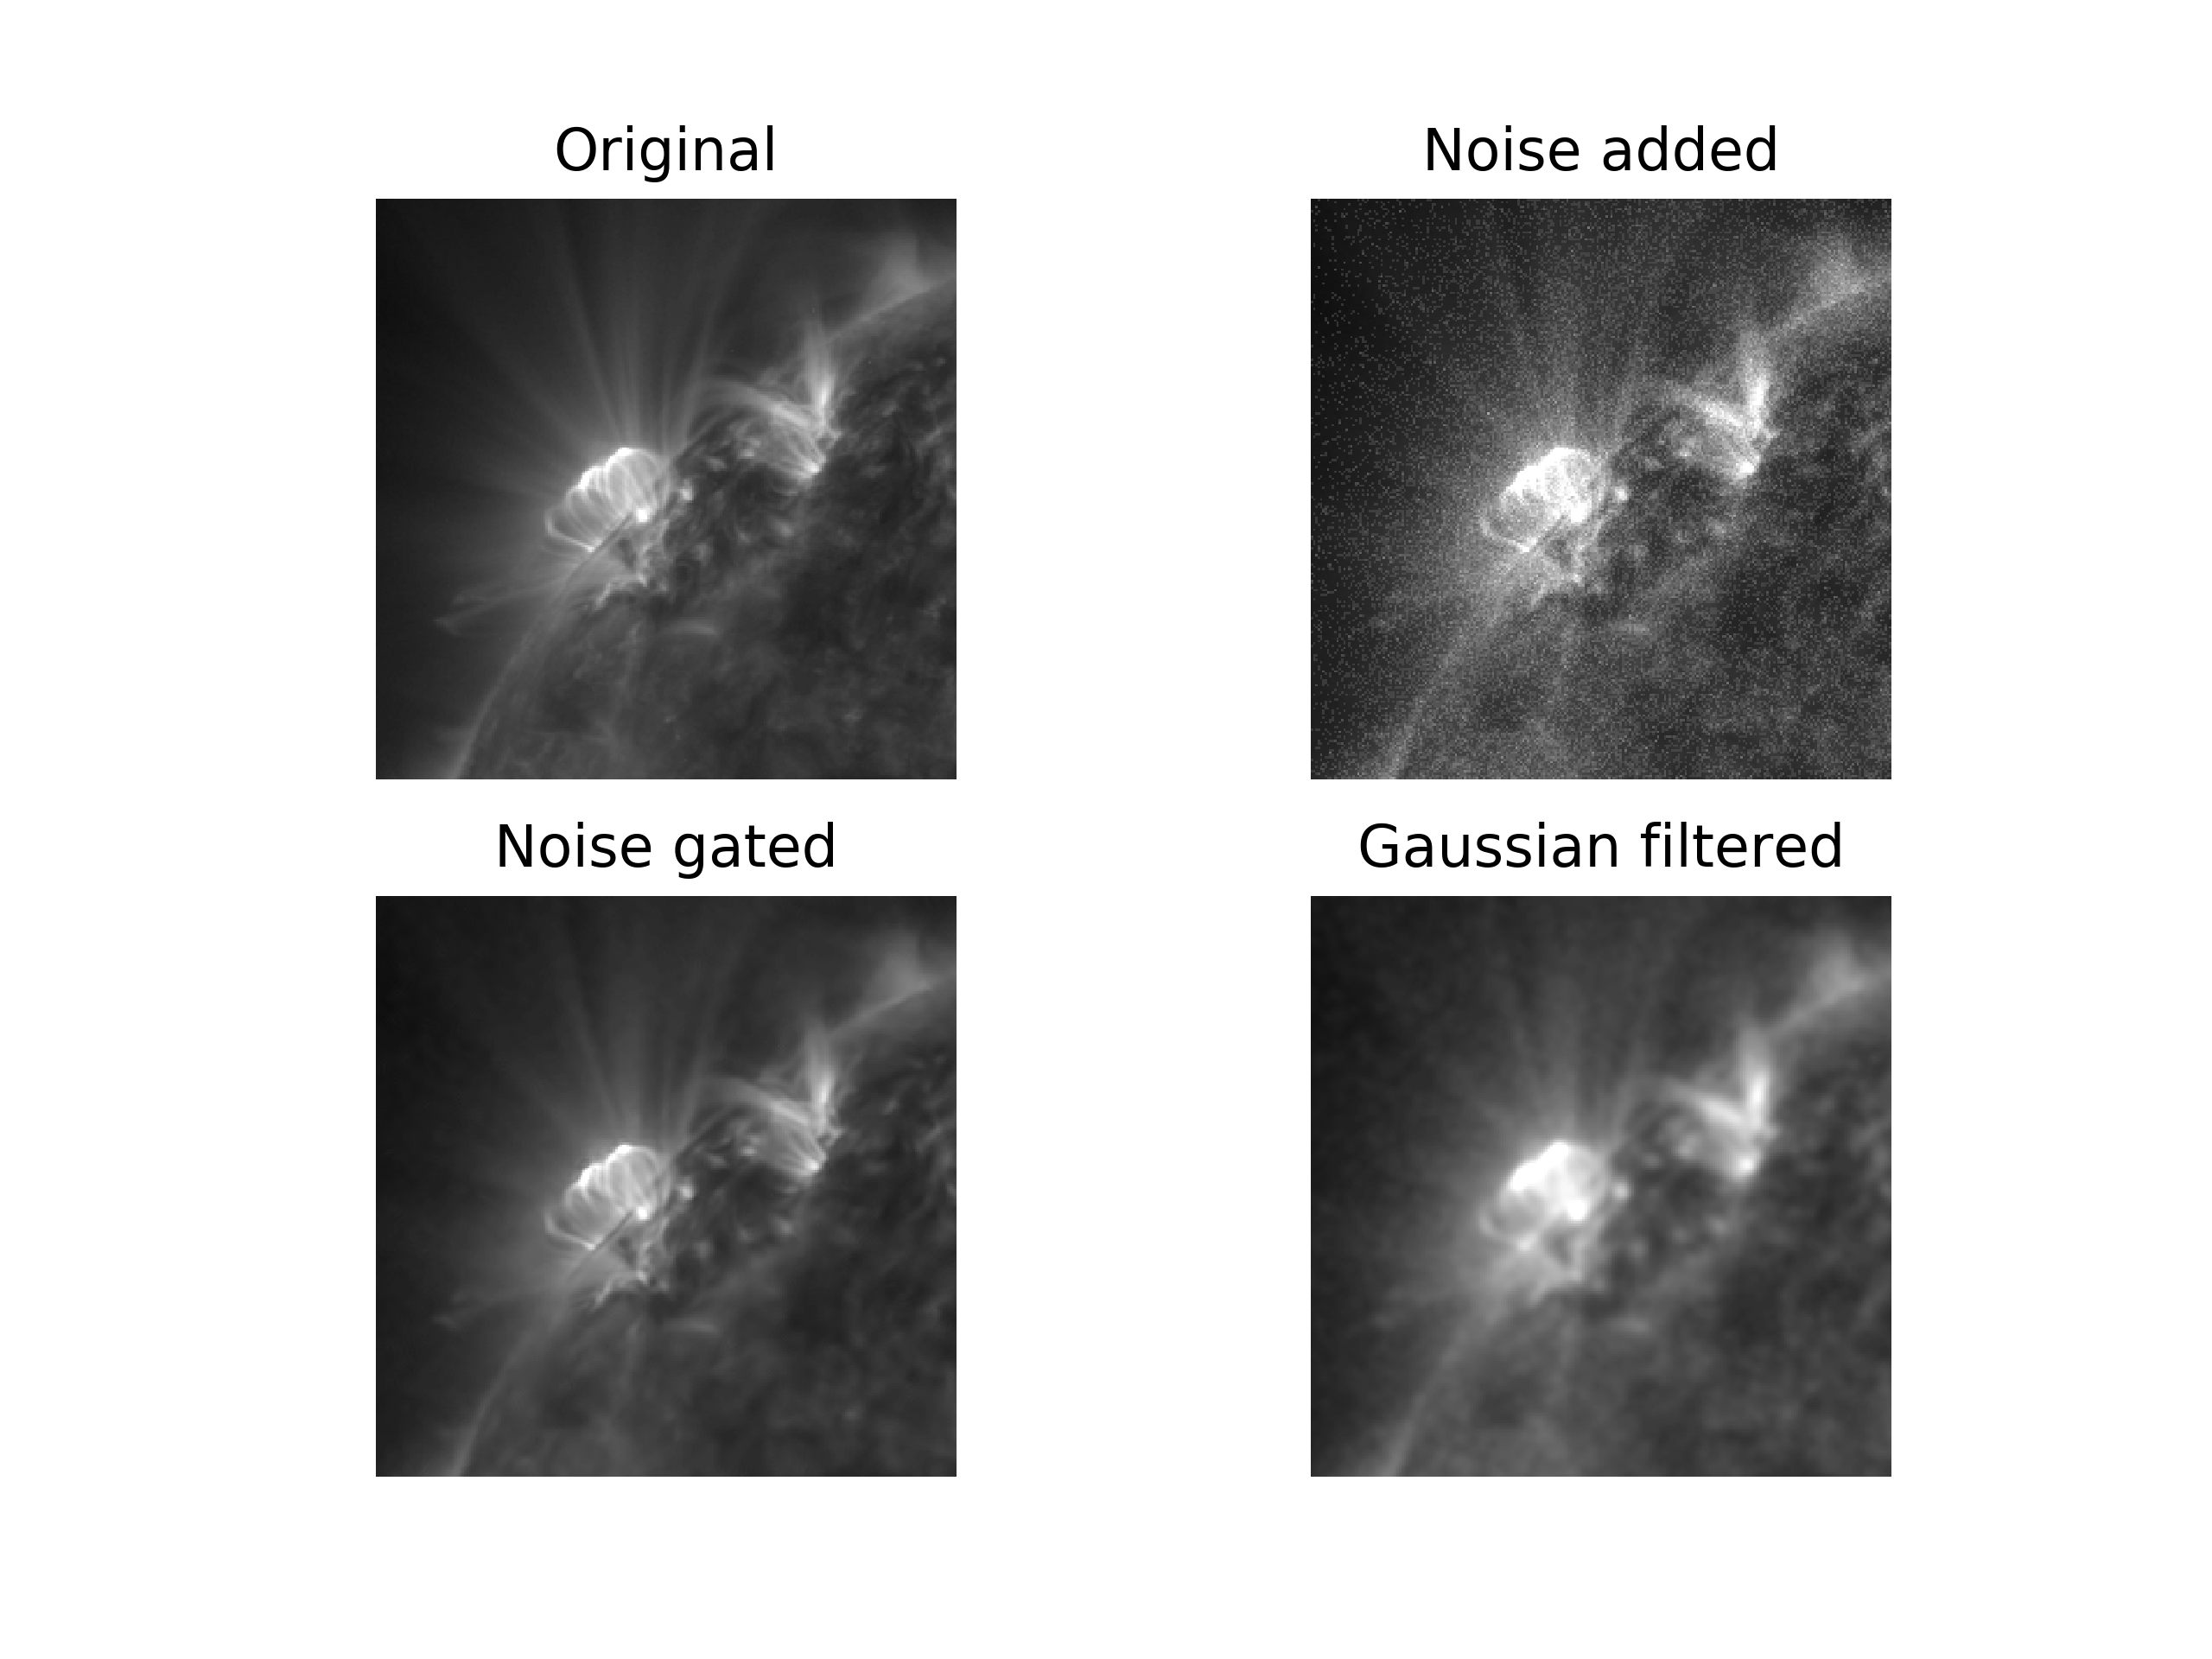
\includegraphics[scale=0.8]{noise-gate.png}
    \caption{{\bf Effectiveness of noise-gating} The upper left is a good image, no cleaning necessary. However, images like the upper right, dominated by shot noise, are typical for the 94 angstrom channel. This image is created by taking the image on the upper left and adding Poisson noise with a signal-to-noise ratio of 2. The algorithm still performs even if it's worse, although some artifacts appear. DeForest's algorithm was applied to create the cleaned image on the bottom left. This can be compared to simply smoothing the image to decrease the noise as in the bottom right, a typical alternative procedure.}
    \label{fig:noise-gate-example}
 \end{center}
\end{figure}

\section{Normalization of data}

\section{Spatial features}

\section{\halpha inclusion}\label{sec:halphainclusion}

\chapter{Applications} \label{ch:application}

\section{Database building} \label{sec:database}

\section{Fractal dimension and class properties} \label{sec:fractal}

\chapter{Conclusion} \label{ch:conclusion}

\section{Summary}

\section{Future work}

\subsection{Stability over solar cycles}

%%%%%%%%References %%%%%%%%%%
\bibliographystyle{acm}
\bibliography{references}
%%%%%%%% End References %%%%%%
\end{document}
